%%%%%%
%
% $Autor: Wings $
% $Datum: 2020-01-18 11:15:45Z $
% $Pfad: githubtemplate/Template/Presentations/Template/rename.tex $
% $Version: 4620 $
%
%
% !TeX encoding = utf8
% bibtex
%
%%%%%%






\documentclass[10pt, a4paper]{beamer}

%Metadaten
\title{Artificial Intelligence with Arduino Portenta H7}

\subtitle{Real-time Object Detection with Vision Shield}
%\institution{University of Applied Science Hochschule Emden/Leer}
\author{Vatsal Mahajan}
%\date{\today}
\date{\today}

% siehe hesader.tex Zeile 10-16 zum Aktivieren der Notes
% Kommentare stehen in \notes{} und können im 2-screen-mode genutzt werden
%%%%%%
%
% $Autor: Wings $
% $Datum: 2020-01-18 11:15:45Z $
% $Pfad: githubtemplate/Template/Presentations/Template/slides/header.tex $
% $Version: 4620 $
%
%
% !TeX encoding = utf8
% !TeX root = Rename
%
%%%%%%


%Packages
\usepackage[utf8]{inputenc} %Für Umlaute, da BibLaTeX
\usepackage[german]{babel}
\usepackage{amsmath}
\usepackage{amsfonts}
\usepackage{amssymb}
\usepackage{colortbl}
\usepackage{cancel} %'\cancel{}', '\bcancel{}' und '\xcancel{}'

%%%%%%%%%2-Screen%%%%%%%%%%%%%%%%%%%%%%%%%%%%%%%%%%%%%%%%%%%%
\usepackage{pgfpages} 
%%%%Kommentiert für Beamer
%%%%Aktiv für Notes
%\setbeameroption{show notes on second screen=bottom}
%\setbeameroption{second mode text on second screen=bottom}
%%%%%%%%%%%%%%%%%%%%%%%%%%%%%%%%%%%%%%%%%%%%%%%%%%%%%%%%%%%%%

%Für Grafiken
\usepackage{tikz}
\usetikzlibrary{mindmap}
\usepackage{gnuplottex}
\usepackage{pgf}
\usepackage{colortbl} 
\usetikzlibrary{calc}
\usetikzlibrary{shapes,arrows} %Für Flowchart
\usetikzlibrary{shapes.geometric} %Für Flowchart
\usepackage{scalefnt}
\usetikzlibrary{decorations.markings} %Für => pfeile
\usetikzlibrary{calc,patterns,decorations.pathmorphing,decorations.markings}
%Für urls in Quellen
\usepackage{url}
%Für Diagramme (autotools)
%\usepackage{graphicx}
%\usepackage{graphviz}

%\usepackage[
%  backend=biber,
%  style=alphabetic,
%  sorting=ynt
%]{biblatex}

\usepackage[natbib=true,style=alphabetic,backend=bibtex,useprefix=true]{biblatex}

%Formatierungen
\mode<presentation>
\setbeamertemplate{headline} 
{%
\begin{beamercolorbox}[rounded=true, center]{bgcolor}
\begin{columns}[T]
\begin{column}{9cm}
{\color{gray}\begin{tiny}Hochschule Emden/Leer\end{tiny}} \\ 
{\color{gray}\begin{tiny}Department of Electrical and Computer Engineering\end{tiny}} \\ 
{\color{gray}\begin{tiny}Industrial Informatics\end{tiny}} \\
%{\color{gray}\begin{tiny}Innovationsforum MSR\end{tiny}}
\end{column}
\begin{column}{2cm}

\includegraphics[scale=0.25]{img/technik.jpg}
\end{column}
\end{columns}
\end{beamercolorbox}
 }
\insertsectionhead
\insertsubsectionhead
\usetheme{default}
\useinnertheme[shadow=true]{rounded}
\usebackgroundtemplate
{%
      \rule{0pt}{\paperheight}%
      \hspace*{\paperwidth}%
      \makebox[0pt][r]{
\includegraphics[width=\paperwidth]{img/hintergrund2.png}}
 }

\definecolor{HSELhellblau}{RGB}{138,198,203}
\definecolor{HSELblau}{RGB}{0,59,95}
\usecolortheme[named=HSELblau]{structure}
 \newcommand{\topline}{%
  \tikz[remember picture,overlay] {%
    \draw[HSELhellblau] ([yshift=-0.9cm]current page.north west)
             -- ([yshift=-0.9cm,xshift=\paperwidth]current page.north west);}}
\setbeamertemplate{section}[numbered]


\newcommand{\STANDARD}[2]
{
  \mode<presentation>%
  {%
     \begin{frame}[allowframebreaks]{#1} #2 \end{frame}
  }%
  \mode<article>
  {
    \fcolorbox{AliceBlue}%{Bisque} %{BlanchedAlmond}
    {LightGrey} %{Beige}   %{AliceBlue}
    {
      \begin{minipage}{\textwidth}{\bf #1} #2  \end{minipage}
      
      
    }%
    
    \medskip
    \hrulefill
  }
}

\newcommand{\MYNOTE}[1]
{
  \mode<presentation>%
  {%
     %\note{#1}
     \only<article>{#1}
  }%
  \mode<article>
  {
    #1
  }
}

% ------------
% sectionframe
% ------------
%
% #1  Der Name der section.
%
\newcommand{\sectionframe}[1]%
{%
	\begin{frame}
		\Huge
		\begin{center}
			#1 
		\end{center}
	\end{frame}%
}

\newcommand{\Mysection}[1]%
{%
  \section{#1}%
  
  \sectionframe{#1}%
}

\usepackage{listings}

% Farben für Syntax-Highlighting
\definecolor{dkgreen}{rgb}{0,.6,0}
\definecolor{dkblue}{rgb}{0.655,0.113,.364}
\definecolor{dkyellow}{cmyk}{0,0,.8,.3}

\definecolor{parameterc}{rgb}{.4,0,.6}
\definecolor{typec}{rgb}{0,0.525,.702}
\definecolor{stringc}{rgb}{0,.5019,.5019}
\definecolor{keywordc}{rgb}{.6549, .1137, .3647}
\definecolor{commentc}{rgb}{.5882, .5960, .5882}
\definecolor{textc}{rgb}{.2,.2,.2}

\lstdefinestyle{all}{
	alsoletter={-},
	frame=single, 	% top,frame=bottom,
	numbers=none,
	numberstyle=\tiny\color{textc},
	basicstyle=\linespread{0.9}\ttfamily\footnotesize\color{textc},
	tabsize=4,
	showstringspaces=false,
	captionpos=t,
	rulecolor=\color{lightgray!40},
	keywordstyle=\color{keywordc},
	stringstyle=\color{stringc},
	commentstyle=\color{commentc},
	breaklines=true,
	escapechar="!",
	postbreak=\mbox{\textcolor{green}{$\hookrightarrow$}\space},
}

\lstdefinestyle{bashstyle}{
	style=all,
	keywords=[2]{-y, --no-install-recommends, --allow-change-held-packages, --allow-downgrades, --fetch-keys, -n, --version, --params, -c, -i, -O, --upgrade, --no-cache-dir, --extra-index-url, --show, -s, -m},
	keywordstyle=[2]\color{parameterc},
	morekeywords = {ln,choco,pip,pip3,apt,apt-key,apt-get,apt-mark,add-apt-repository,wget,mktemp,dpkg,dpkg-query,echo,>>,rm,tegrastats, systemctl},
	deletekeywords={local,LOCAL},
}

\lstdefinestyle{pythonstyle}{
	style=all,
	morekeywords={as},
	keywords=[2]{True, False, None},
	keywordstyle=[2]\color{typec},
	alsoletter={_},
	keywords=[3]{max_workspace_size_bytes, precision_mode, maximum_cached_engines, use_calibration, optimizer, loss, input_shape, from_logits, metrics, batch_size, epochs, validation_data, activation, use_calibration, filters, kernel_size, pool_size, units},
	keywordstyle=[3]\color{parameterc},
	deletekeywords={compile,COMPILE},
}

\lstdefinestyle{inlinestyle}{
	style=all,
	breaklines        = true,
	breakatwhitespace = true,
	breakindent       = 2ex,
	escapechar        = *,
	numbers           = left,
	postbreak=,
}
\lstdefinelanguage{MyBash} {
	language = Bash,
	style=bashstyle,
}

\lstdefinelanguage{MyPython} {
	language = Python,
	style=pythonstyle,
}


\definecolor{PythonColor}{rgb}{0,0.5,1.}
\newcommand{\PYTHON}[1]{\textcolor{PythonColor}{\texttt{#1}}}
\definecolor{PythonColorHighLite}{rgb}{0.5,0,1.}
\newcommand{\PYTHONHL}[1]{\textcolor{PythonColorHighLite}{\texttt{#1}}}
\definecolor{MapleColor}{rgb}{1,0,0}
\newcommand{\MapleCommand}[1]{\textcolor{MapleColor}{\texttt{#1}}}
\definecolor{ShellColor}{rgb}{0,1,1.}
\newcommand{\SHELL}[1]{\textcolor{ShellColor}{\texttt{#1}}}
\definecolor{FileColor}{rgb}{1,0,1.}
\newcommand{\FILE}[1]{\textcolor{FileColor}{\texttt{#1}}}

\addbibresource{Documents/MyLiterature.bib} %Import the bibliography file

\begin{document}


\setbeamercolor{bgcolor}{fg=black,bg=white}
\selectlanguage{german}
\setbeamertemplate{footline}{%
\vspace*{-.1cm}\hspace*{.5cm}
\scriptsize{%
%%\hspace*{1pt}\insertauthor
%%\inserttitle
\hspace{325pt}\insertframenumber/\inserttotalframenumber}
}

\STANDARD{}
{
  \titlepage
}

\MYNOTE
{
  \ldots
}



\STANDARD{}
{
\tableofcontents[hideallsubsections]
}

\MYNOTE
{
  \ldots
}

\setbeamercovered{transparent}

%%%%%%
%
% $Autor: Wings $
% $Datum: 2020-01-18 11:15:45Z $
% $Pfad: githubtemplate/Template/Presentations/Template/slides/quellen.tex $
% $Version: 4620 $
%
%
% !TeX encoding = utf8
% !TeX root = Rename
%
%%%%%%

\Mysection{Quellen}


\begin{frame}[allowframebreaks]{Quellen}
 
  
  Nachfolgend werden die Quellen der Bilder angegeben, 
  die für diese Präsentation in ihrer ursprünglichen Form oder modifiziert verwendet worden sind.

  \nocite{*}

  {\tiny 
%  \bibliographystyle{unsrturl}
    \printbibliography %Prints bibliography
  }

\end{frame}

\begin{frame}{Components}
	
	
	\begin{block}{Description}
	The project involves the following components:
	\begin{itemize}
		\item \textbf{Arduino Portenta H7:} The core microcontroller unit providing processing power and resources for AI algorithms.
		\item \textbf{Vision Shield:} An accessory for the Portenta H7, equipped with a camera module and display for image capture and processing.
		\item \textbf{AI Model:} A pre-trained model deployed on the Portenta H7 for object detection tasks.
	\end{itemize}
\end{block}

\end{frame}

\begin{frame}

\begin{block}{Role}
	\begin{itemize}
		\item \textbf{Arduino Portenta H7:} Provides computational power and interfaces with the Vision Shield.
		\item \textbf{Vision Shield:} Captures live video frames and displays annotated results.
		\item \textbf{AI Model:} Analyzes video frames for real-time object detection and display detected objects on the Vision Shield's built-in display in real-time.
	\end{itemize}
\end{block}

  \nocite{*}

{\tiny 
	%  \bibliographystyle{unsrturl}
	\printbibliography %Prints bibliography
}

\end{frame}

%\begin{frame}{Figure}
	
	\begin{columns}
		\column{0.5\textwidth}
		\centering
		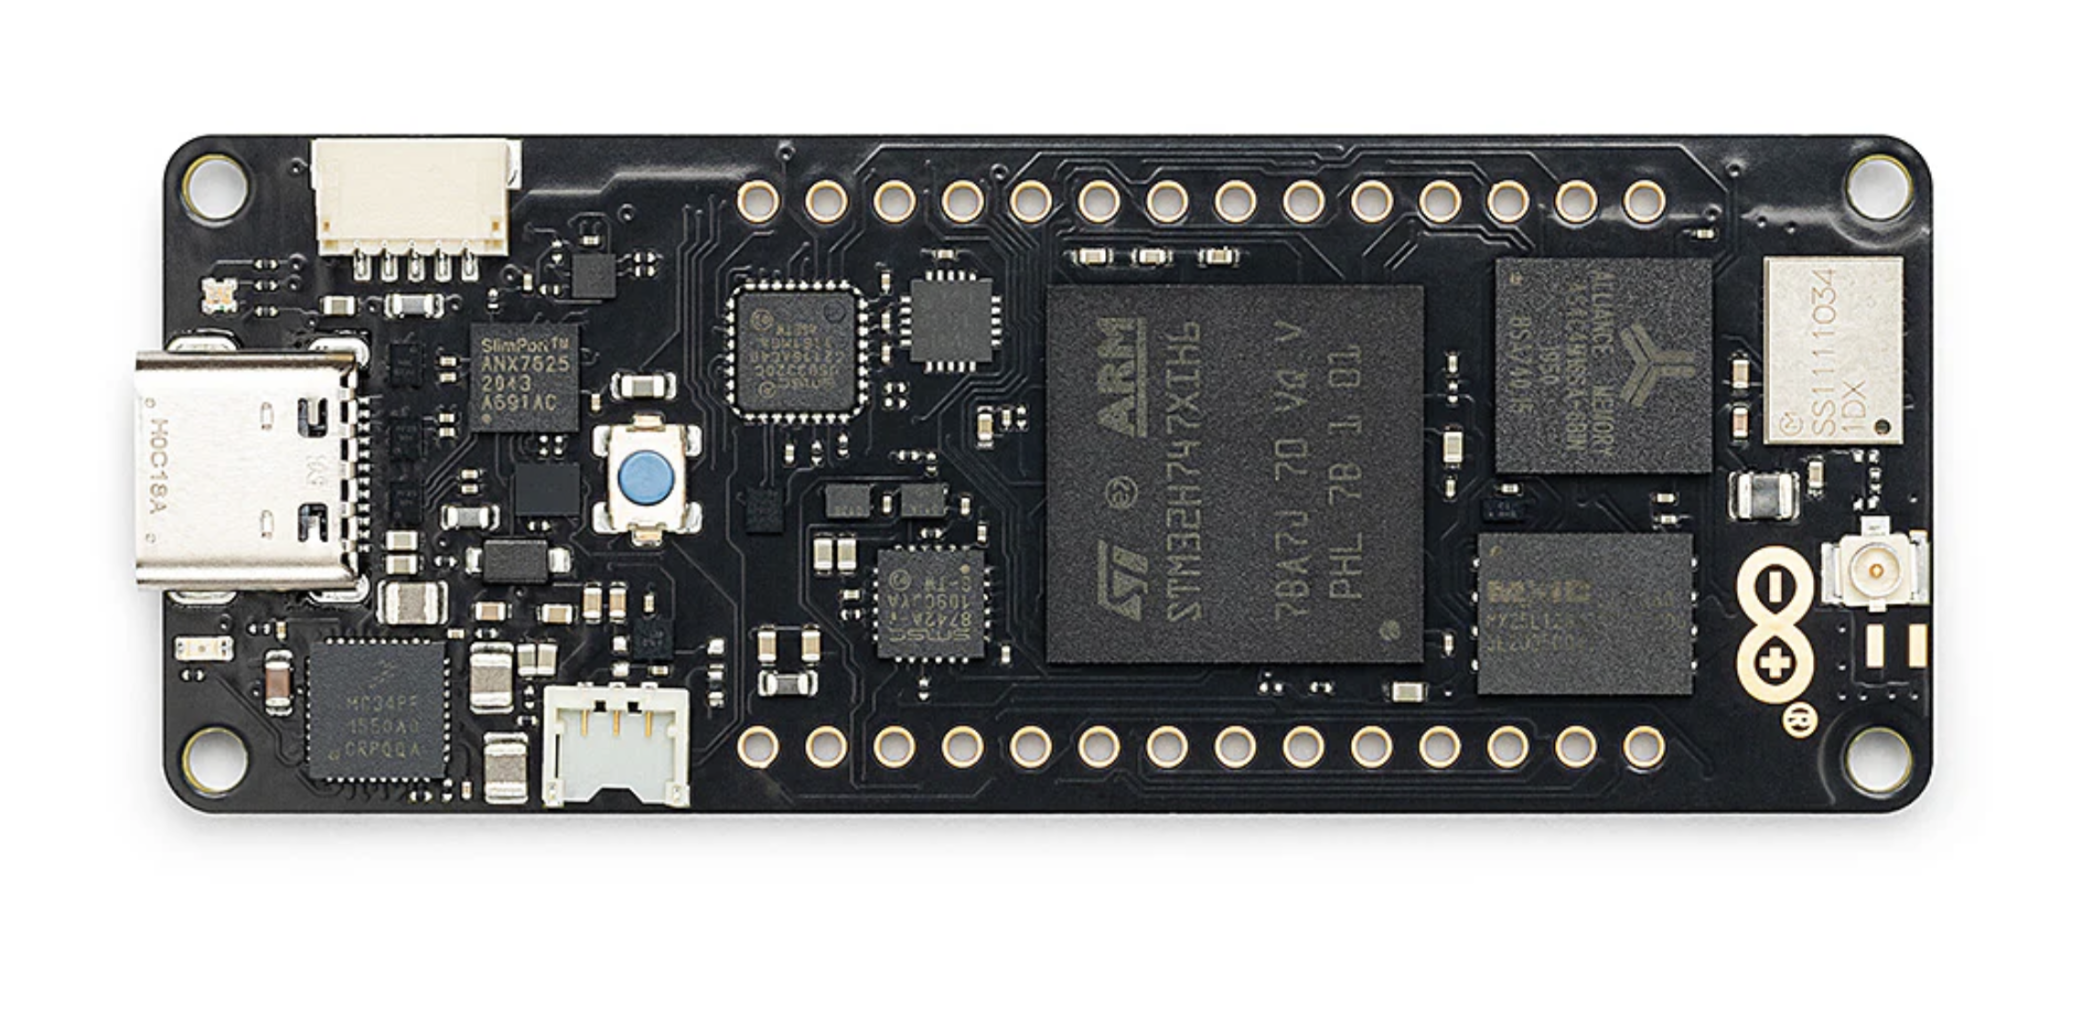
\includegraphics[width=\textwidth]{images/ArduinoPortentaH7.png}
		\captionof{figure}{Arduino PortentaH7}
		
		\column{0.5\textwidth}
		\centering
		\includegraphics[width=\textwidth]{images/{PortentaVisionShield.png}
		\captionof{figure}{PortentaH7 Vision Shield}
	\end{columns}
	
\end{frame}

%%%%%%
%
% $Autor: Wings $
% $Datum: 2020-01-18 11:15:45Z $
% $Pfad: githubtemplate/Template/Presentations/Template/slides/rename.tex $
% $Version: 4620 $
%
%
% !TeX encoding = utf8
% !TeX root = Rename
%
%%%%%%



\Mysection{Trajectory Planning}

\STANDARD{Introduction}
{ 
	
 \begin{frame}{Introduction}
 	
 	
 	\begin{block}{Project Overview}
 		This presentation focuses on the project titled \textbf{Real-time Object Detection with a Vision Shield}, which demonstrates the integration of artificial intelligence (AI) with embedded systems.
 	\end{block}
 	
 	
 	\begin{block}{Project Objectives}
 		\begin{itemize}
 			\item Develop a system for real-time object detection using Arduino Portenta H7 and Vision Shield.
 			\item Implement AI algorithms on embedded devices for efficient and accurate object detection.
 		\end{itemize}
 	\end{block}
 	
 	\begin{block}{Importance}
 		Real-time object detection has applications in surveillance, industrial automation, robotics, and IoT, among others.
 	\end{block}
 	
 	\nocite{*}
 	
 	{\tiny 
 		%  \bibliographystyle{unsrturl}
 		\printbibliography %Prints bibliography
 	}
 	
 \end{frame}

\STANDARD{Trajectory Planning}
{ 

  \textbf{Aufgabe}: Beziehung zwischen Zeit und Position finden

  \textbf{Synonyme}: Path Planning, Motion Planning

  Unterscheidung hier:

  \begin{itemize}
    \item Geometrie (Path): Position der Aktoren ohne Zeitinformation
    \item Trajektorie (Trajectory): Position, Geschwindigkeit, Beschleunigung und Ruck als Funktion über die Zeit
  \end{itemize}
% Seite 2 Trajectory generation for a four axis robot with linear kinematics - S.N. van den Brink - DCT 2005.69
%With a trajectory we indicate the position, velocity, acceleration and jerk profiles of every actuator as a function of time.
%With a path, the subsequent positions of every actuator without time information is indicated

\textbf{Vereinfachung}

  \begin{itemize}
    \item Eindimensionale Trajektorie: $q=q(t)$
          \\Definiert durch eine Skalar-Funktion
    \item Mehrdimensionale Trajektorie: $\textbf{p}=\textbf{p}(t)$
          \\Definiert durch eine Vektor-Funktion
  \end{itemize}

  \textbf{Einschränkung}: zunächst nur eindimensionale Trajektorien; \cite{Piegl:1997}
}

\STANDARD{Trajectory Planning}
{ 

  $q_0$: Startposition

  $q_1$: Zielposition

  \begin{figure}[!h]
    \centering
    \begin{tikzpicture}

\draw  (-3,0.5) node[left] (v1) {$q_0=q(t_0)$} ellipse (0.05 and 0.05);
\draw  (-0.5,0.5) node[right] (v2) {$q_1=q(t_1)$} ellipse (0.05 and 0.05);
\draw[-latex]  (-3,0.5) -- node[above]{$q=q(t)$} (-0.5,0.5);
\end{tikzpicture}
  \end{figure}
}

\section{Notation}
\STANDARD{Notation}
{ 


  Position

  \begin{equation}
    q(t)
  \end{equation}

  Geschwindigkeit (Velocity)

  \begin{equation}
    v(t) 
    = \dot{q}(t) 
    = \frac{d}{dt} q(t)
  \end{equation}

  Beschleunigung (Acceleration)

  \begin{eqnarray}
    a(t) 
    = \dot{v}(t) = \frac{d}{dt} v(t) 
    = \ddot{q}(t) = \frac{d^2}{dt^2} q(t)
  \end{eqnarray}

  Ruck (Jerk)

  \begin{eqnarray}
    j(t) 
    = \dot{a}(t) = \frac{d}{dt} a(t)
    = \ddot{v}(t) = \frac{d^2}{dt^2} v(t)
    = q^{(3)}(t) = \frac{d^3}{dt^3} q(t)
    %= \dddot{q}(t) = \frac{d^3}{dt^3} q(t)
  \end{eqnarray}
}


\section{Bang-Bang-Control}

\STANDARD{Bang-Bang-Control}
{ 

  \textbf{Prozess}: Positionierung

  \textbf{Aufgabe}: Positionieren in möglichst kurzer Zeit

  \textbf{Ansatz}: Höchstmögliches ausreizen der limitierende(n) Größe(n)

  \textbf{Grenzen}: Limitierende Größen (Constraints) ergeben sich

  \begin{itemize}
    \item durch den Motor
          
          über die Höchstdrehzahl wird $v_{max}$ festgelegt
          
          über das Drehmoment wird $a_{max}$ festgelegt
    \item durch die Dynamik des mechanischen Systems
          
          über Steifigkeit/Nachgiebigkeit wird $j_{max}$ festgelegt
    \item durch die Geometrie wird festgelegt, ob
          
          $j_{max}$, $a_{max}$ und $v_{max}$ überhaupt erreicht werden können
      \begin{itemize}
        \item da \textbf{hier} nur eindimensionale Trajektorien betrachtet werden, ist nur die \textbf{Weglänge} der begrenzende Faktor
        \item bei mehrdimensionalen Trajektorien ist die Krümmung ein weiterer begrenzender Faktor
      \end{itemize}
  \end{itemize}
}

\STANDARD{Water Taxi}
{
  \begin{center}
    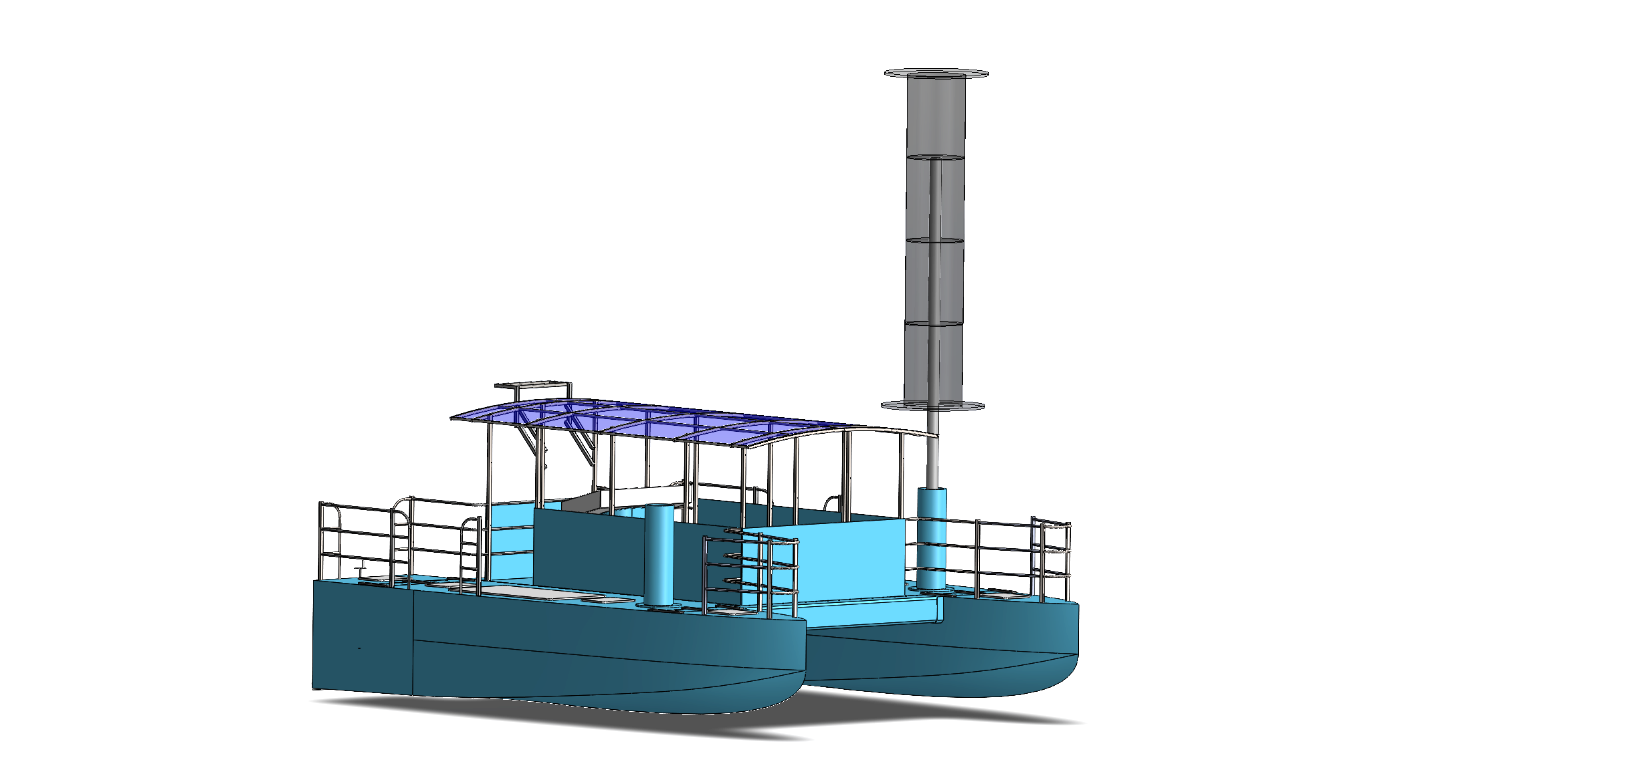
\includegraphics[width=\textwidth]{images/WaterTaxi}
  \end{center}	
}

\STANDARD{3D-Printer}
{
	\begin{center}
		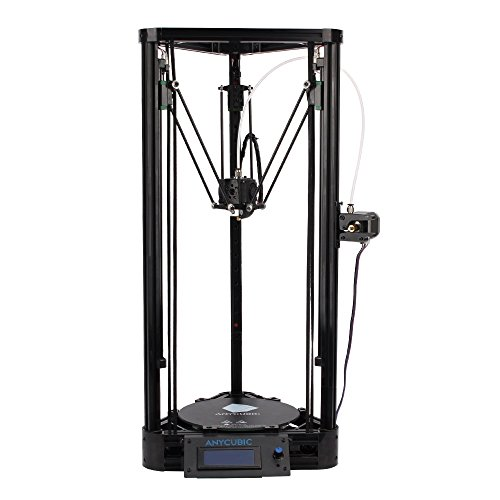
\includegraphics[height=0.8\textheight]{images/Rostock}
	\end{center}	
}


\STANDARD{3D-Printer}
{
  Der Datenstruktur \PYTHON{MyStructure} aus der Datei \FILE{MyStructure.py} ist sehr interessant.	
}


\begin{frame}[fragile]{Code}

%, numbers=left, caption={Konstruktion eines Keras-Sequential-Modells}, label={src:kerasmodel}]

  \begin{lstlisting}[language=Python]
import tensorflow as tf
from tensorflow.keras import datasets, layers, models

MODEL = models.Sequential()
  \end{lstlisting}

\end{frame}

\begin{frame}[fragile]{Code}

  \lstinputlisting[language=Python, firstnumber=1]{Code/PDFExtractTable/PDFExtractTable.py}
\end{frame}


\STANDARD{}
{
  \begin{columns}
    \begin{column}{0.35\textwidth}
      \begin{block}{~~~~~~Thank you}
        \centering
        for your attention
      \end{block}
    \end{column}
  \end{columns}
}

\MYNOTE{Ja, \textbf{Vielen} Dank, für Ihre Aufmerksamkeit}



\end{document}
